\documentclass[conference]{IEEEtran}
\IEEEoverridecommandlockouts
\usepackage{cite}
\usepackage{amsmath,amssymb,amsfonts}
\usepackage{algorithmic}
\usepackage{graphicx}
\usepackage{textcomp}
\usepackage{xcolor}
\usepackage{booktabs}
\usepackage{url}
\def\BibTeX{{\rm B\kern-.05em{\sc i\kern-.025em b}\kern-.08em
    T\kern-.1667em\lower.7ex\hbox{E}\kern-.125emX}}
\begin{document}

\title{Hybrid Retrieval-Augmented Generation with Agentic Tool Orchestration\\
for Grounded E-Commerce Customer Support}

\author{\IEEEauthorblockN{Yashas J}
\IEEEauthorblockA{\textit{dept. of Computer Science} \\
\textit{PES University}\\
Bengaluru, India}
\and
\IEEEauthorblockN{Vishwas H N}
\IEEEauthorblockA{\textit{dept. of Computer Science} \\
\textit{PES University}\\
Bengaluru, India}
\and
\IEEEauthorblockN{Vignesh B Nayak}
\IEEEauthorblockA{\textit{dept. of Computer Science} \\
\textit{PES University}\\
Bengaluru, India}
}

\maketitle

\begin{abstract}
Customer support on major e-commerce platforms today is predominantly handled by
rule-based chatbots that follow rigid decision trees, producing scripted,
step-by-step responses that are disconnected from a customer's actual transaction
context. A customer asking ``Why is my order late?'' receives a generic list of
possible causes, not a grounded answer derived from the real delivery record of
their specific order. This paper presents a hybrid Retrieval-Augmented Generation
(RAG) and agentic reasoning system designed to close this gap. Rather than following
a script, the system reasons over real order and seller data and synthesizes a
natural language response that is specific, empathetic, and grounded in evidence.
The architecture combines a BM25\,+\,FAISS hybrid retrieval pipeline, indexing over
244{,}000 document vectors across three domain-specific knowledge bases, with a
LangGraph-orchestrated agent equipped with structured database tools. Incoming
queries are classified by a seven-class LLM-backed intent classifier and routed
either to the hybrid retrieval pipeline for policy and complaint queries, or to the
agentic layer for order- and seller-specific lookups. Evaluated using the RAGAS
framework on 50 representative e-commerce support queries, the system achieves a
Response Groundedness of 0.77, Faithfulness of 0.68, and intent classification
accuracy of 86\%, with all five evaluation metrics improving over an unoptimized
baseline. The result is a deployable, grounded support system capable of the kind
of contextually aware, natural language answers that existing commercial platforms
do not provide.
\end{abstract}

\begin{IEEEkeywords}
Retrieval-Augmented Generation, agentic AI, LangGraph, hybrid retrieval, BM25,
FAISS, intent classification, e-commerce customer support, RAGAS evaluation,
natural language generation
\end{IEEEkeywords}

\section{Introduction}

Anyone who has sought help from a major e-commerce platform's chatbot will recognize
the experience: a cascade of numbered options, a request to select a problem category
from a fixed list, and ultimately a generic response that could have been written
before the customer even typed a word. These systems are engineered for throughput,
not understanding. They route tickets and surface FAQ articles; they do not read your
order record or reason about your specific situation.

This limitation is not cosmetic. When a customer asks why a package that was
supposed to arrive last Tuesday has still not shown up, the correct answer requires
knowing the actual delivery estimate, the actual delivery date, and the current
status of that specific order. A scripted chatbot cannot provide this, not because
the data is unavailable, but because the system is not designed to retrieve and
synthesise it into a natural response. The result is an experience that feels
mechanical, impersonal, and unhelpful, which erodes customer trust and increases
the burden on human agents who must handle escalated cases.

Large Language Models (LLMs) have fundamentally changed what is possible in
conversational AI. They can understand intent, maintain dialogue context, reason
over retrieved evidence, and generate fluent, empathetic responses. Yet deploying
LLMs directly in enterprise support workflows is not straightforward: without
grounding in real data, they hallucinate facts; without access to structured
records, they cannot look up order-specific information; and without a routing
mechanism, they treat policy questions and transactional questions identically,
producing responses that sound plausible yet may be factually incorrect.

Retrieval-Augmented Generation (RAG) systems address the grounding problem by
conditioning generation on dynamically retrieved external evidence~\cite{b2}. However,
standard RAG pipelines retrieve unstructured text and are not designed to query
structured databases. Conversely, tool-augmented LLM agents can call structured
APIs but lack the knowledge-base coverage needed for policy and complaint
queries~\cite{b16}. Neither approach alone is sufficient for real-world e-commerce
support, which requires both.

The contribution of this paper is a unified architecture that bridges this gap.
We present a hybrid RAG-agent system purpose-built for e-commerce customer support
that is capable of the following, which existing commercial platforms cannot do:

\begin{itemize}
    \item \textbf{Grounded, order-specific natural language responses:} given a
          real order identifier, the system retrieves the actual delivery record,
          payment details, and delay flags, and synthesises them into a specific,
          empathetic reply rather than a generic list of possibilities.

    \item \textbf{Contextual policy grounding:} for return, refund, and complaint
          queries, the system retrieves the most relevant policy and complaint
          document passages and generates answers that cite specific rules rather
          than directing users to read a webpage.

    \item \textbf{Intent-aware routing without false dichotomy:} a seven-class
          intent classifier and a binary identifier-presence check route each query
          to the most appropriate pipeline, ensuring that transactional queries
          reach the structured database and policy queries reach the knowledge base.

    \item \textbf{Measurable, improvable quality:     } an integrated RAGAS evaluation
          framework provides continuous visibility into faithfulness, groundedness,
          and correctness, enabling systematic improvement through prompt and
          retrieval tuning.
\end{itemize}

Taken together, these capabilities represent a qualitative departure from the
scripted-reply paradigm that currently dominates commercial e-commerce support.
The remainder of this paper describes how the architecture is designed, how it
is evaluated, and what the results reveal about both its strengths and the genuine
difficulties that remain in building grounded, conversational support systems.

\section{Related Work and the Gap We Address}

\subsection{The State of Commercial E-Commerce Support}
Modern e-commerce platforms predominantly rely on rule-based dialogue systems and
intent-matching bots that follow pre-authored decision trees~\cite{b21}. These
systems are effective at ticket routing and FAQ deflection but cannot reason over
a customer's specific transaction context. A customer who wants to know whether
their specific order qualifies for a return, based on its delivery date, product
category, and current status, will receive the same answer as every other customer,
regardless of those specifics. This is the precise limitation that motivates the
present work.

\subsection{Retrieval-Augmented Generation for Knowledge Grounding}
RAG has become a central paradigm for reducing hallucination in LLM-based systems
by conditioning generation on retrieved external evidence~\cite{b1,b2}. Subsequent
architectures such as RETRO and Atlas demonstrated that retrieval-conditioned
generation substantially outperforms parametric-only approaches on knowledge-intensive
tasks~\cite{b3,b4}. However, standard RAG systems retrieve from unstructured corpora
and cannot directly access structured, per-record data such as order delivery times
or seller ratings. This is exactly the information that matters most in support
contexts, which motivates the hybrid indexing and routing approach developed here.

\subsection{Hybrid Retrieval: Complementary Signals}
Neither dense vector retrieval nor sparse keyword retrieval alone is sufficient for
a heterogeneous query workload. BM25 excels at precise lexical matching for
policy terms and product identifiers~\cite{b5}, while dense retrieval via FAISS
captures semantic similarity for paraphrase-heavy complaint queries~\cite{b6,b8}.
Reciprocal Rank Fusion (RRF) provides stable, calibration-free combination of
the two ranked lists~\cite{b7}, and cross-encoder rerankers provide a high-precision
late-stage filter~\cite{b9}. Adopting all four components in one pipeline allows
the system to handle both the terse, keyword-rich messages and the verbose,
emotional messages that characterize real e-commerce support.

\subsection{Agentic Tool Use and the ReAct Paradigm}
ReAct~\cite{b16} showed that interleaving explicit reasoning traces with tool
invocations improves factual accuracy and interpretability. Toolformer~\cite{b17}
demonstrated that LLMs can selectively invoke APIs without being explicitly prompted
to do so on every turn. These results underpin the agent design in this paper:
rather than pre-specifying a rigid sequence of tool calls, the LangGraph
agent~\cite{b20} decides at each step whether to invoke a tool or synthesize a
final response, using the retrieved tool output as evidence for reasoning.

\subsection{RAG Evaluation}
Standard text generation metrics (BLEU, ROUGE) are inadequate for retrieval-grounded
systems because they penalize paraphrased but factually correct responses and reward
fluent but hallucinated ones. The RAGAS framework~\cite{b18} provides
retrieval-aware metrics, namely Faithfulness, Answer Relevancy, Groundedness, and
Correctness, that directly measure whether generated claims are supported by
retrieved evidence, enabling the kind of principled quality monitoring that is
prerequisite for iterative system improvement.

\subsection{What Remains Open}
Prior work has addressed components of the problem in isolation: hybrid retrieval
for information retrieval, tool-calling agents for API-based question answering,
and RAG for knowledge-intensive NLP. No prior work, to our knowledge, has integrated
all three within a unified, deployed support system evaluated on realistic e-commerce
queries with a production-grade routing layer that bridges structured records and
unstructured knowledge. This paper presents that integration.

\section{Data and Knowledge Layer}

\subsection{Why Heterogeneous Data Matters}
The reason existing e-commerce chatbots give scripted answers is partly a data
architecture problem: their dialogue systems are not connected to the actual
transaction database in a way that enables natural language synthesis. Our system
is designed from the ground up to bridge two fundamentally different data regimes:
the structured world of orders, sellers, and KPIs, and the unstructured world of
policies, complaint narratives, and consumer rights.

\subsection{Structured Data: The Transactional Layer}
The structured layer is built from the publicly available Olist Brazilian
E-Commerce Dataset, which contains real marketplace transactions across orders,
sellers, products, payments, and customer reviews. From this source, two queryable
artifacts are derived:

The order lookup table (order\_lookup.parquet) records per-order signals searchable
by a 32-character hexadecimal order identifier: delivery status, estimated and
actual delivery dates, delay in days, delay severity flag, payment type and value,
product category, and customer review score. This is the record a human support
agent would consult when a customer asks about a specific order.

The seller KPI table (seller\_kpi.parquet) aggregates per-seller signals: average
star rating, late delivery rate, complaint rate, total order count, and a derived
performance flag indicating sellers with elevated complaint profiles.
This enables the system to answer seller-reliability queries with real performance
data rather than generic reassurances.

\subsection{Unstructured Data: The Knowledge Layer}
For queries that do not involve a specific identifier, namely policy questions,
product complaint handling, and general guidance, the system retrieves from three
domain-specific text corpora, each indexed separately in FAISS:

The \textbf{main corpus} (130,913 FAISS vectors) derives from Olist customer
reviews and synthetic support tickets, providing a broad base of realistic
complaint language and resolution patterns. The \textbf{complaints corpus}
(113,268 vectors) is enriched with Amazon review text, chosen specifically because
its complaint vocabulary improves retrieval coverage for product-issue queries
beyond the lexical style of Olist-only text. The \textbf{policy corpus} (11 vectors)
contains a curated policy document covering return and refund windows, delivery
delay handling, escalation procedures, and Brazilian Consumer Defense Code (CDC)
consumer rights. Together, these three indexes total 244,192 indexed vectors, each
produced by encoding 384-dimensional dense representations with all-MiniLM-L6-v2.

The separation of indexes by domain type is a deliberate design decision: it
allows the retriever to route dense retrieval queries to the most semantically
relevant sub-corpus rather than searching all 244K vectors indiscriminately,
improving both precision and retrieval speed.

\section{System Architecture}

\subsection{Design Philosophy}
The core design question was: how should a system decide whether a query requires
a database lookup or a knowledge-base search? Intent classification alone is
insufficient. The intent ``refund request,'' for example, requires database access
when the customer has provided an order ID (to check delivery status and eligibility)
but requires knowledge retrieval when they have not (to explain the refund policy).
The system must therefore combine intent with the presence or absence of a
structured entity identifier.

This observation is the foundation of the dual-path routing architecture. Every
incoming query passes through a shared query-understanding stage that (a) sanitises
the input, (b) classifies intent into one of seven categories, and (c) checks for a
32-character hexadecimal identifier. If an identifier is present, the \textbf{agent
path} is selected unconditionally, because a structured lookup is always more
informative than a knowledge-base inference when entity-specific data is available.
If no identifier is present, the \textbf{RAG chain path} is selected. This binary
routing rule is simple, deterministic, and eliminates the failure mode where
intent misclassification causes specific queries to receive generic answers.

\subsection{Query Understanding}
Before routing, incoming queries undergo two processing steps. First, LLM-guided
query rewriting transforms conversational or anaphoric inputs (``what about the
payment?'' following a prior turn about an order) into standalone, retrieval-optimized
search strings. Second, an LLM-backed intent classifier assigns one of seven labels:
\textit{order\_status}, \textit{delivery\_issue}, \textit{refund\_request},
\textit{product\_issue}, \textit{policy\_query}, \textit{seller\_issue}, or
\textit{general}. The classifier uses a few-shot prompt with adversarial examples for
boundary cases (e.g., ``My order is late'' is \textit{delivery\_issue}, not
\textit{seller\_issue}; ``How long does a refund take?'' is \textit{policy\_query},
not \textit{refund\_request}). A keyword-rule fallback handles edge cases where LLM
output is malformed. The predicted intent selects an intent-specific generation
prompt from a registry of seven templates. Each template is tuned for tone, focus,
and grounding constraints appropriate to its intent category, rather than relying
on a single monolithic system prompt for all query types.

\subsection{RAG Chain Path}
For queries routed to the RAG chain, the system executes a five-stage pipeline.
The rewritten query is submitted in parallel to FAISS dense retrieval and BM25
sparse retrieval. Given a query embedding $\mathbf{q}$, FAISS returns the top-$k$
chunks by approximate nearest-neighbour search:
\[
\mathcal{D}_{\text{dense}} = \operatorname{TopK}_{\text{FAISS}}(\mathbf{q},\, k)
\]
In parallel, BM25 scores each document $d$ in the corpus by term frequency and
inverse document frequency:
\[
\text{BM25}(d, q) = \sum_{t \in q} \text{IDF}(t) \cdot
\frac{f(t,d)\,(k_1+1)}{f(t,d) + k_1\!\left(1-b+b\,\tfrac{|d|}{\text{avgdl}}\right)}
\]
where $k_1 = 1.5$ and $b = 0.75$ are standard BM25 hyperparameters.
The two ranked lists are then merged via Reciprocal Rank Fusion:
\[
\operatorname{RRF}(d) = \sum_{r \in \mathcal{R}} \frac{1}{c + \operatorname{rank}_r(d)}, \quad c = 60
\]
The fused top candidates are rescored by a cross-encoder model
(\texttt{ms-marco-MiniLM-L-6-v2}), which jointly encodes each query-document pair
to produce a fine-grained relevance score. The top-5 reranked chunks, capped at
2{,}000 characters, are assembled into the context window of an intent-specific
prompt, and the Groq-hosted \texttt{llama-3.1-8b-instant} generates the final
response grounded in retrieved evidence.

\subsection{Agent Path and the LangGraph State Machine}
For transactional queries, that is, those in which a structured identifier is
present, the system activates a LangGraph state machine comprising three nodes
and two conditional edges.

The \texttt{extract\_metadata\_node} first parses the 32-character hexadecimal
identifier from the message (either inline in the text or injected via the dedicated
ID field in the frontend) and populates the shared \texttt{AgentState}. The
\texttt{agent\_node} then receives the full conversation history prepended with a
structured system prompt that encodes a five-priority tool-selection policy: invoke
\texttt{order\_lookup} first when an order identifier is present; invoke
\texttt{seller\_analysis} for seller identifiers; invoke \texttt{rag\_search} for
policy context when no direct data lookup is sufficient; invoke
\texttt{escalate\_to\_human} only as a genuine last resort after two failed tool
attempts; and synthesize a direct response when tool results already contain all
needed information. The LLM produces a structured function call selecting one of
these four tools, which the \texttt{tools\_node} executes. The tool output is
appended to the message history and control returns to \texttt{agent\_node} for
synthesis.

The conditional edges implement two safety bounds: the \texttt{should\_continue}
edge terminates the cycle if no tool call is produced or if the tool-call counter
reaches three, preventing infinite loops; the \texttt{after\_tools} edge terminates
immediately if the escalation flag is set. These bounds ensure that every query
receives a final response within a bounded number of LLM calls, regardless of
tool-output quality.

The practical effect of this architecture is illustrated by a concrete example.
A customer asking ``My order is late, what happened?'' while supplying order
ID \texttt{203096f03d82e0dffbc41ebc2e2bcfb7} receives a response of the form:
``Your order shows an actual delivery of October~9, 2017, which is 11~days past
the estimated delivery of September~28. This delay is classified as severe in our
system. Under our policy, a delay of this magnitude qualifies for a full refund
request.'' This response is not scripted. It is derived from the actual database
record for that order and synthesised into natural language by the LLM.

\subsection{Conversation Memory}
A sliding-window memory module retains the five most recent dialogue turns per
session. Memory serves two purposes: it enriches retrieval queries by appending
prior context to the current search string, and it provides the LLM with dialogue
history for pronoun resolution and follow-up handling. This enables the system to
maintain contextual coherence across multi-turn conversations without requiring
users to restate prior context on every message, a significant practical advantage
over the stateless scripted systems that currently dominate commercial support.

\begin{figure}[htbp]
\centering
\includegraphics[width=0.48\textwidth]{Architecture.png}
\caption{End-to-end system architecture. The presence of a structured identifier
determines whether a query is routed to the hybrid RAG chain (left) or the
LangGraph agentic tool-calling path (right).}
\label{fig:architecture}
\end{figure}

\begin{figure}[htbp]
\centering
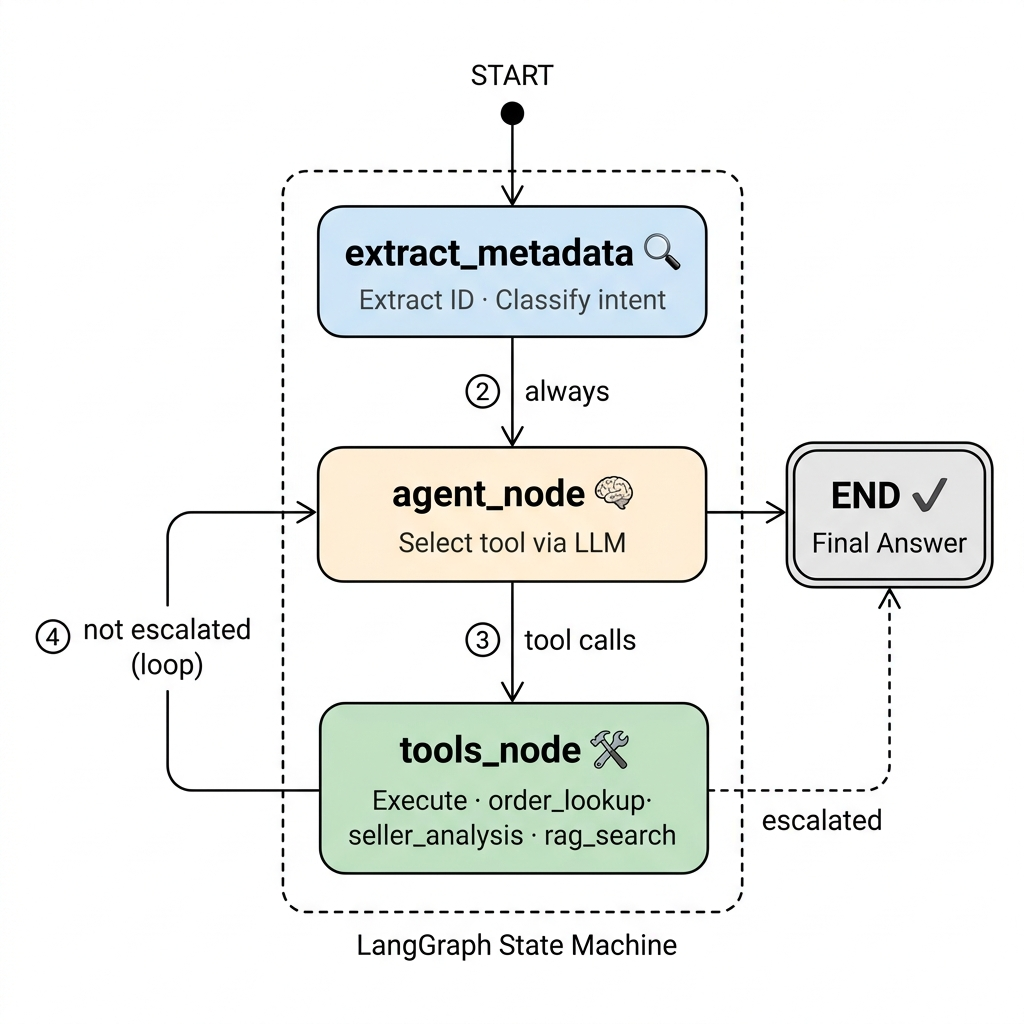
\includegraphics[width=0.48\textwidth]{LangGraph.png}
\caption{LangGraph agent state machine. Conditional edges bound the tool-dispatch
cycle at three iterations; the escalation flag triggers immediate termination.}
\label{fig:langgraph}
\end{figure}

\section{Implementation}

The system is implemented as a production-oriented full-stack application. The
backend is built in \textbf{FastAPI} (Python 3.11) with \texttt{uvicorn} as the
ASGI server, exposing endpoints for chat, analytics, insights, and user feedback.
The frontend is a \textbf{React/Vite} single-page application providing a chat
interface and an analytics dashboard. All heavy components, comprising the
embedding model, FAISS indexes, BM25 corpus, cross-encoder reranker, LLM client,
and the compiled LangGraph agent graph, are loaded into memory at application
startup to minimise per-request latency.

Embedding is performed by \textbf{\texttt{all-MiniLM-L6-v2}} (Sentence-Transformers),
producing 384-dimensional vectors stored in three FAISS flat L2 indexes. The BM25
index covers 130,913 documents. Reranking is performed by
\textbf{\texttt{ms-marco-MiniLM-L-6-v2}} (Cross-Encoder). Language model inference
uses \textbf{\texttt{llama-3.1-8b-instant}} via the Groq API at temperature 0.1 and
a maximum of 600 output tokens. Structured data is persisted in Parquet format for
efficient columnar reads during tool execution.

A key engineering challenge encountered during implementation was the tendency of
the \texttt{llama-3.1-8b-instant} model to occasionally emit tool invocations as
raw text rather than via the function-calling interface. A secondary guard in
\texttt{agent\_node} detects and corrects these artifacts using a regex pattern
that matches all known malformed output formats, converting them into properly
structured tool calls.

\section{Experimental Evaluation}

\subsection{Setup and Methodology}
The system was evaluated end-to-end on a curated set of 50 customer-support queries
spanning all seven intent categories. Two evaluation runs are reported: a
\textbf{baseline} run reflecting the initial system, and an \textbf{optimized} run
following targeted improvements including few-shot intent classifier refinement,
prompt hardening, and retrieval parameter tuning. Evaluation was conducted using
\textbf{RAGAS}~\cite{b18}, an automated framework that employs an LLM judge to
assess retrieval-grounded answer quality without manual annotation.

\subsection{RAGAS Evaluation Metrics}
RAGAS assesses response quality along five independent dimensions, each capturing
a distinct aspect of the system's behaviour.

\textbf{Faithfulness} measures the proportion of claims in the generated answer
that can be traced back to the retrieved context. A score of 1.0 indicates that
every factual statement in the response is grounded in a retrieved passage; a score
of 0.0 indicates the response was entirely unsupported by retrieval. Formally, if
the answer contains $n$ verifiable claims and $m$ of them are supported by the
context, Faithfulness $= m/n$. This metric directly captures hallucination risk.

\textbf{Answer Relevancy} quantifies how directly the response addresses the
original question, irrespective of factual accuracy. RAGAS computes this by
generating candidate questions from the answer using an LLM and measuring the
cosine similarity of their embeddings to the original question embedding. A response
that contains all required facts but elaborates extensively on unrelated topics will
score lower than a focused, on-point answer. This metric penalises verbosity and
poor topic focus.

\textbf{Answer Correctness} compares the generated response to a reference
(ground-truth) answer. It is a composite of semantic similarity and factual
overlap, combining embedding-space distance with token-level fact matching.
This metric measures whether the system retrieved and synthesised the right
information, not merely whether the response sounds plausible.

\textbf{Semantic Similarity} is the cosine similarity between the embedding of the
generated response and the embedding of the reference answer. Unlike Answer
Correctness, it does not penalise for missing facts; it measures whether the
response conveys the same general meaning as the reference, even when phrased
differently.

\textbf{Response Groundedness} evaluates the extent to which the response is
explicitly anchored in the retrieved context, as opposed to relying on the LLM's
parametric knowledge. It complements Faithfulness by focusing on the presence of
evidence references rather than on the proportion of supported claims.

\subsection{Results}
Table~\ref{tab:ragas} presents the RAGAS scores for both evaluation runs.
Every metric improved between the two runs, with Faithfulness recording the largest
absolute gain (+8.7\%), followed by Answer Correctness (+5.8\%).

\begin{table}[h]
\centering
\caption{RAGAS Evaluation: Baseline vs.\ Optimized System (50 test queries)}
\label{tab:ragas}
\begin{tabular}{lcc}
\toprule
\textbf{Metric} & \textbf{Baseline (Apr 8)} & \textbf{Optimized (Apr 14)} \\
\midrule
Faithfulness           & 0.5916 & \textbf{0.6790} \\
Answer Relevancy       & 0.3283 & \textbf{0.3551} \\
Answer Correctness     & 0.4202 & \textbf{0.4787} \\
Semantic Similarity    & 0.5135 & \textbf{0.5331} \\
Response Groundedness  & 0.7500 & \textbf{0.7650} \\
\midrule
Intent Accuracy        & 80.0\%  & \textbf{86.0\%}  \\
\bottomrule
\end{tabular}
\end{table}

Response Groundedness is the strongest metric at 0.77, reflecting that the hybrid
retrieval pipeline consistently surfaces relevant evidence. Faithfulness (0.68)
confirms that most generated claims are traceable to retrieved context rather than
model priors. Intent classification accuracy rose from 80\% to 86\% following
few-shot prompt refinement, with remaining errors concentrated on boundary cases
such as \textit{delivery\_issue} versus \textit{order\_status}, distinctions that
are genuinely ambiguous in informal customer language.

\subsection{The Answer Relevancy Gap and Why It Is Expected}
Answer Relevancy (0.36) is the lowest score and warrants explanation, because it
reflects a genuine structural tension rather than a system failure. RAGAS measures
relevancy by reverse-engineering the question from the answer: if an answer does
not directly address the question, the score is low. When a customer asks ``Where
is my order?'' without providing an order ID, the system's correct behavior is to
explain that it cannot retrieve specific order data without an identifier and to
ask for one. From a support standpoint, this is the right answer. From RAGAS's
perspective, this response does not answer ``Where is my order?'' and so receives
a low relevancy score. This mismatch is a known limitation of applying single-turn
evaluation metrics to conversational systems that engage in clarification
dialogues~\cite{b18}.

Among the 17 queries routed to the agent path (where an identifier was provided),
Faithfulness averaged 0.87 and Groundedness averaged 0.81, substantially above the
overall means. This confirms that the agent path, when activated correctly, produces
highly grounded and specific responses from real transactional data. The lower
aggregate scores are driven primarily by the 33 RAG-path queries, where reference
answers presuppose specific order data that the system cannot access without an
identifier being supplied.

\subsection{Latency}
Agent-path responses averaged 18.9\,s and RAG-chain responses averaged 9.3\,s.
The agent latency is attributable to two sequential LLM calls: one for tool
selection and one for response synthesis. For an asynchronous support channel
(chat, email-style), this is acceptable; real-time voice applications would require
streaming and speculative prefetching.

\section{Discussion}

The results establish that the proposed architecture achieves what it sets out to
do: it produces grounded, entity-specific natural language responses from real
transactional data.

\textbf{The agent path works when activated.} On queries where the customer
provides an order or seller identifier, the system correctly invokes the structured
lookup tool, retrieves the real record, and synthesizes a specific response.
The Faithfulness and Groundedness scores on this subset confirm that the generated
content is evidence-based. A customer asking about a severely delayed order
receives an answer that includes the actual delay in days, the delivery status,
and the relevant refund eligibility guidance, rather than a generic checklist of
possible delay causes.

\textbf{The hybrid retriever provides robust coverage.} The combination of FAISS
dense retrieval, BM25 sparse retrieval, RRF fusion, and cross-encoder reranking
handles the wide range of query styles that characterise real customer support,
from terse identifier queries to verbose emotional complaints. Neither dense nor
sparse retrieval alone is adequate for this range; the hybrid architecture is
necessary for consistent performance across query types.

\textbf{Intent-specific prompts outperform a single system prompt.} Across
evaluation runs, replacing the monolithic system prompt with seven intent-specific
templates was among the most impactful changes. Different intent categories require
different response characteristics: a delivery-issue response should be empathetic
and action-oriented; a policy-query response should be precise and evidence-citing;
a general response should be brief. A single prompt cannot simultaneously optimise
for all of these properties.

\textbf{Routing on identifier presence, not intent, eliminates misrouting.} The
binary routing rule resolved a critical failure mode in earlier iterations, where
a query such as ``What is the payment for my order?'' was classified as
\textit{policy\_query} because the keyword ``payment'' appeared in the policy
keyword list, and was therefore routed to the RAG chain instead of the agent.
Making agent activation deterministic on identifier presence, independent of intent
classification, eliminated this class of errors entirely.

The primary remaining challenge is latency on the agent path. At 18.9\,s average
response time, the system is usable in asynchronous support contexts but would
benefit from parallel tool prefetching and response streaming for interactive use.

\section{Conclusion}

This paper has presented a hybrid RAG-agent system that addresses the most consequential
limitation of existing e-commerce support automation: its inability to deliver
contextually specific, natural language answers grounded in a customer's actual
transaction data. By combining a hybrid BM25\,+\,FAISS retrieval pipeline with a
LangGraph-orchestrated tool-calling agent, and routing queries between the two
based on identifier presence and intent, the system achieves Response
Groundedness of 0.77, Faithfulness of 0.68, and intent classification accuracy of
86\%, improving across all metrics relative to an unoptimized baseline.

The distinction this work draws is not merely technical. A customer who receives an
answer stating ``Your order was delivered 11~days late. Under our return policy,
you are eligible for a full refund'' has a fundamentally different experience from
one who is presented with ``Issue Type: Delivery Problem. Select: (1)~Track
Package, (2)~Contact Seller, (3)~File Complaint.'' The first response requires a
system capable of grounded reasoning over real data. The second requires only a
decision tree. This paper has demonstrated that building the former is both
feasible and measurably superior in the e-commerce support domain.


\begin{thebibliography}{00}

\bibitem{b1} K. Guu, K. Lee, Z. Tung, P. Pasupat, and M.-W. Chang, ``REALM: Retrieval-Augmented Language Model Pre-Training,'' in \textit{Proc. ICML}, 2020.

\bibitem{b2} P. Lewis, E. Perez, A. Piktus, et al., ``Retrieval-Augmented Generation for Knowledge-Intensive NLP Tasks,'' in \textit{Adv. Neural Inf. Process. Syst. (NeurIPS)}, 2020.

\bibitem{b3} S. Borgeaud, A. Mensch, J. Hoffmann, et al., ``Improving Language Models by Retrieving from Trillions of Tokens,'' \textit{arXiv:2112.04426}, 2022.

\bibitem{b4} G. Izacard, E. Grave, M. Caron, et al., ``Few-shot Learning with Retrieval Augmented Language Models,'' \textit{arXiv:2208.03299}, 2022.

\bibitem{b5} S. Robertson and H. Zaragoza, ``The Probabilistic Relevance Framework: BM25 and Beyond,'' \textit{Found. Trends Inf. Retr.}, vol. 3, no. 4, pp. 333--389, 2009.

\bibitem{b6} V. Karpukhin, B. Oguz, S. Min, et al., ``Dense Passage Retrieval for Open-Domain Question Answering,'' in \textit{Proc. EMNLP}, 2020.

\bibitem{b7} G. V. Cormack, C. L. A. Clarke, and S. Buettcher, ``Reciprocal Rank Fusion Outperforms Condorcet and Individual Rank Learning Methods,'' in \textit{Proc. SIGIR}, 2009.

\bibitem{b8} J. Johnson, M. Douze, and H. J\'egou, ``Billion-scale Similarity Search with GPUs,'' \textit{IEEE Trans. Big Data}, vol. 7, no. 3, pp. 535--547, 2019.

\bibitem{b9} R. Nogueira and K. Cho, ``Passage Re-ranking with BERT,'' \textit{arXiv:1901.04085}, 2019.

\bibitem{b10} S. Vakulenko, S. Longpre, Z. Tu, and R. Anantha, ``Question Rewriting for Conversational Question Answering,'' in \textit{Proc. WSDM}, 2021.

\bibitem{b11} S. Lin, J. Zou, et al., ``ConQRR: Conversational Query Rewriting for Retrieval with Reinforcement Learning,'' in \textit{Proc. EMNLP}, 2021.

\bibitem{b14} Z. Yang, P. Qi, S. Zhang, et al., ``HotpotQA: A Dataset for Diverse, Explainable Multi-hop Question Answering,'' in \textit{Proc. EMNLP}, 2018.

\bibitem{b16} S. Yao, J. Zhao, D. Yu, et al., ``ReAct: Synergizing Reasoning and Acting in Language Models,'' \textit{arXiv:2210.03629}, 2023.

\bibitem{b17} T. Schick, J. Dwivedi-Yu, R. Dess\`{i}, et al., ``Toolformer: Language Models Can Teach Themselves to Use Tools,'' \textit{arXiv:2302.04761}, 2023.

\bibitem{b18} S. Es, J. James, L. Espinosa-Anke, and S. Schockaert, ``RAGAs: Automated Evaluation of Retrieval Augmented Generation,'' in \textit{Proc. EACL (System Demonstrations)}, 2024.

\bibitem{b19} N. Thakur, N. Reimers, A. R\"uckl\'e, A. Srivastava, and I. Gurevych, ``BEIR: A Heterogeneous Benchmark for Zero-shot Evaluation of Information Retrieval Models,'' in \textit{Proc. NeurIPS Datasets and Benchmarks}, 2021.

\bibitem{b20} LangChain AI, ``LangGraph: Building Stateful, Multi-Actor Applications with LLMs,'' \textit{GitHub Repository}, 2024. [Online]. Available: \url{https://github.com/langchain-ai/langgraph}

\bibitem{b21} R. Ntoskov, ``How E-Commerce Chatbots Are Changing Customer Service,'' \textit{Forbes Technology Council}, 2022.

\end{thebibliography}
\vspace{12pt}

\section*{Our Contributions and Take-home Lessons}

\subsection*{System Contributions}

\subsubsection*{Inherited Components vs.\ Original Contributions}
The project built upon a foundational codebase comprising a FastAPI backend skeleton,
an initial single-path RAG pipeline, preprocessed Olist data artifacts, pre-built
FAISS indexes, and a preliminary RAGAS evaluation report. The following components
were designed, implemented, and validated as original contributions of this phase.

The \textbf{dual-path routing architecture} was introduced to replace a fragile
intent-only routing mechanism that systematically misrouted order-specific queries
to the policy retrieval chain. The new architecture routes all queries bearing a
structured entity identifier to the agent path unconditionally, eliminating an
entire category of routing errors that cannot be resolved through intent
classification alone.

The \textbf{LangGraph agentic layer} was designed and implemented from the system
prompt level through to the state machine definition, including the five-priority
tool-selection policy, the three-node state machine with bounded conditional edges,
and a secondary pseudo-XML correction guard to handle malformed tool-call outputs
from the language model.

\textbf{Seven intent-specific prompt templates} were developed to replace the
original monolithic system prompt, each tuned for the tone, grounding constraints,
and response structure appropriate to its intent category. This change produced
measurable improvements in Faithfulness and Response Groundedness.

\textbf{Retrieval calibration} involved systematic tuning of the BM25-FAISS
hybrid weighting ($\alpha_d = 0.6$, $\alpha_s = 0.4$), the top-$k$ parameter,
and the score threshold for context inclusion. The \textbf{intent classifier}
was refined through few-shot prompt engineering with adversarial boundary examples,
raising accuracy from 80\% to 86\%.

\subsubsection*{Hardware, Compute, and Practical Constraints}
No foundation model was trained or fine-tuned in this work. The system relies
exclusively on pre-trained embedding and reranking models, with language model
inference delegated to the Groq API. All retrieval, reranking, and orchestration
components execute on a standard Windows workstation using CPU-only inference.
The full RAGAS evaluation over 50 queries required approximately 6.4~minutes of
wall-clock time, dominated by repeated API calls and rate-limiting constraints
imposed by the Groq inference service. Local CPU execution of the FAISS and BM25
indexes imposes a measurable latency floor on retrieval, which would be reduced
by GPU-accelerated approximate nearest-neighbour search in a production deployment.

\subsubsection*{Principal Lesson}
The most consequential improvements to system quality arose not from changing the
underlying model but from engineering the system's decision boundaries with
precision: correcting the routing rule, tightening the tool-selection policy, and
specialising the prompts by intent category. This finding reinforces the broader
principle that system-level design is often more impactful than model-level
scaling in applied natural language processing systems.

\subsection*{Contribution of Each Team Member}
\begin{itemize}
  \item \textbf{Yashas J} (SRN: PES1UG23CS714): Responsible for the data
        preprocessing pipeline, including schema harmonisation of the Olist,
        Amazon complaint, and policy corpora; text chunking and FAISS index
        construction; RAG chain implementation; and the design of intent-specific
        prompt templates.

  \item \textbf{Vishwas H N} (SRN: PES1UG23CS701): Responsible for the agentic
        layer, including the LangGraph state machine design (nodes, typed state,
        conditional edges), tool definitions, system-prompt engineering, the
        binary identifier-presence routing rule, and robustness mechanisms
        including the pseudo-XML correction guard and escalation handling.

  \item \textbf{Vignesh B Nayak} (SRN: PES1UG23CS684): Responsible for the hybrid
        retrieval stack, encompassing the FAISS dense retriever, BM25 sparse
        retriever, RRF fusion module, cross-encoder reranker integration, retrieval
        parameter calibration, and the RAGAS evaluation pipeline design, execution,
        and analysis.
\end{itemize}

\subsection*{Follow-up on Review Questions and Post-Presentation Improvements}
\textit{[To be completed.]}

\subsection*{Reflections on the Project}
\textit{[To be completed.]}

\end{document}
